\documentclass[a4paper,norsk, 10pt]{article}
\usepackage[utf8]{inputenc}
\usepackage{verbatim}
\usepackage{listings}
\usepackage{graphicx}
\usepackage[norsk]{babel}
\usepackage{a4wide}
\usepackage{color}
\usepackage{amsmath}
\usepackage{float}
\usepackage{amssymb}
\usepackage[dvips]{epsfig}
\usepackage[toc,page]{appendix}
\usepackage[T1]{fontenc}
\usepackage{cite} % [2,3,4] --> [2--4]
\usepackage{shadow}
\usepackage{hyperref}
\usepackage{titling}
\usepackage{marvosym }
%\usepackage{subcaption}
\usepackage{subfig}
\usepackage[noabbrev]{cleveref}
\usepackage{cite}


\setlength{\droptitle}{-10em}   % This is your set screw

\setcounter{tocdepth}{2}

\lstset{language=c++}
\lstset{alsolanguage=[90]Fortran}
\lstset{alsolanguage=Python}
\lstset{basicstyle=\small}
\lstset{backgroundcolor=\color{white}}
\lstset{frame=single}
\lstset{stringstyle=\ttfamily}
\lstset{keywordstyle=\color{red}\bfseries}
\lstset{commentstyle=\itshape\color{blue}}
\lstset{showspaces=false}
\lstset{showstringspaces=false}
\lstset{showtabs=false}
\lstset{breaklines}
\title{AST4320 Assignment 1}
\author{Daniel Heinesen, daniehei}
\begin{document}
\maketitle

\section{Exercise 1}
\subsection{a)}
We have the continuity equation
\begin{equation}
\frac{d\rho_0}{dt} + \rho_0 \nabla \cdot \mathbf{v} = \frac{\partial\rho_0}{\partial t} + \mathbf{v}\cdot \nabla \rho_0 + \rho_0 \nabla \cdot \mathbf{v} = 0.
\end{equation}
Since we have homogeneous universe model, we see that $\nabla \rho \approx 0$, so we get
\begin{equation}
\frac{\partial\rho_0}{\partial t} + \rho_0 \nabla \cdot \mathbf{v} = 0.
\end{equation}
We are assuming a universe that follows Hubble's law $\mathbf{v} = H\mathbf{r} = \frac{\dot{a}}{a}\mathbf{r}$. Since we are in a spherical universe, with a velocity that only depends on the radial direction, we get a divergence of the following form
\begin{equation}
\nabla \cdot \mathbf{v} = \frac{1}{r^2}\frac{\partial (r^2 \cdot v_r)}{\partial r} = \frac{1}{r^2}\frac{\partial (r^3)}{\partial r} = 3,
\end{equation}
which gives us the following for the continuity equation
\begin{equation}
\frac{\partial\rho_0}{\partial t} + 3\frac{\dot{a}}{a}\rho_0 = 0 \Leftrightarrow \frac{d\rho_0}{\rho_0} = -3 \frac{da}{a}.
\end{equation}
Integrating on both sides from $\rho_0(t=t_0) \rightarrow \rho(t)$ and $a_0 = 1 \rightarrow a$ we get
\begin{equation}
\ln \frac{\rho}{\rho_0} = \ln a^{-3} \Leftrightarrow \rho_0(t) = \rho_0(t=t_0)a^{-3}.
\end{equation}
\subsection{b)}
We have the Euler and Poisson equation with the permutations
\begin{equation}
\rho = \bar{\rho} + \delta \rho, \quad \phi = \phi_0 + \delta \phi, \quad v = v_0 + \delta v, \quad p = p_0 + \delta p, \quad \delta = \frac{\delta \rho}{\bar{\rho}}.
\end{equation}
Note that the velocities are vector quantities, but for brevity I have omitted writing them as such here.
\subsubsection{i)}
We start with the Euler equation
\begin{equation}
\frac{dv}{dt} = - \frac{1}{\rho}\nabla p - \nabla \phi.
\end{equation}
We start with the LHS:
\begin{equation}
\frac{dv}{dt} = \frac{\partial v}{\partial t} + v\cdot \nabla v = \frac{\partial v_0 + \delta v}{\partial t} + (v_0 + \delta v)\cdot \nabla (v_0 + \delta v)
\end{equation}
\begin{equation}
= \frac{\partial v_0}{\partial t} + \frac{\partial \delta v}{\partial t} + v_0\cdot \nabla v_0 + \delta v\cdot \nabla v_0 + v_0\cdot \nabla \delta v + \delta v\cdot \nabla \delta v
\end{equation}
\begin{equation}
= \frac{d \delta v}{dt} + \frac{d v_0}{dt} + \delta v \cdot \nabla v.
\end{equation}
In the last step we use that the product of two infinitesimals are more or less zero, and the definition of total derivatives. We can then move on to the RHS:
\begin{equation}
-\frac{1}{\rho}\nabla p - \nabla \phi = -\frac{1}{\bar{\rho} + \delta \rho}\nabla (p_0 + \delta p) - \nabla (\phi_0 + \delta \phi)
\end{equation}
\begin{equation}
= -\frac{1}{\bar{\rho}}\frac{1}{1+\frac{\delta\rho}{\rho_0}}\left(\nabla p_0 + \nabla \delta p\right) - \nabla \phi_0 - \nabla \delta \phi
\end{equation}
\begin{equation}
= -\frac{1}{\bar{\rho}}\nabla p_0 -\frac{1}{\bar{\rho}}\nabla \delta p - \nabla \phi_0 - \nabla \delta \phi.
\end{equation}
In the last step we used that $\delta \rho / \rho_0 << 1$ so that $1/(1+\delta \rho / \rho_0) \approx 1$. Putting all this together, we get
\begin{equation}
\frac{d \delta v}{dt} + \frac{d v_0}{dt} + \delta v \cdot \nabla v. = -\frac{1}{\bar{\rho}}\nabla p_0 -\frac{1}{\bar{\rho}}\nabla \delta p - \nabla \phi_0 - \nabla \delta \phi.
\end{equation}
Knowing that $v_0$, $p_0$, $\bar{\rho}$ and $\phi_0$ have to follow the Euler equation, we can remove half of the term, leaving us with
\begin{equation}
\frac{d \delta v}{dt} + \delta v \cdot \nabla v. =  -\frac{1}{\bar{\rho}}\nabla \delta p  - \nabla \delta \phi.
\end{equation}



\subsubsection{ii)}
We can now look at the Poisson equation:
\begin{equation}
\nabla^2 \phi = 4\pi G\rho.
\end{equation}
Inserting the perturbations we get
\begin{equation}
\nabla^2 (\phi_0 + \delta \phi_0) = 4\pi G(\bar{\rho} + \delta \rho)
\end{equation}
\begin{equation}
\Rightarrow \nabla^2 \phi_0 + \nabla^2\delta \phi_0 = 4\pi G\bar{\rho} + 4\pi G\delta \rho.
\end{equation}
And knowing that $\phi_0$ and $\bar{\rho}$ have to follow the Poisson equation and can be removed, we get
\begin{equation}
\nabla^2 \delta\phi = 4\pi G \delta\rho.
\end{equation}



\section{Exercise 2}
\subsection{a)}
We want to find expressions for $H = \dot{a}/a$. We start with the expression when $(\Omega_{m},\Omega_{\Lambda}) = (1,0)$. We know from the lecture notes that this gives
\begin{equation}\label{eq:o_m=1}
H = 2/3t.
\end{equation}
For the next two combinations, we need to solve the differential equation
\begin{equation}\label{eq:H^2}
H^2 = H_0^2\left[{\Omega_{m}}{a^{-3}} + \Omega_{\Lambda}\right].
\end{equation}
Knowing that $H=\dot{a}/a$ we get
\begin{equation}\label{eq:a_dot}
\dot{a} = H_0\sqrt{\left({\Omega_{m}}{a^{-3}} + \Omega_{\Lambda}\right)}a.
\end{equation}
\begin{equation}
\Rightarrow \frac{da}{a\sqrt{{\Omega_{m}}{a^{-3}} + \Omega_{\Lambda}}} = H_0dt.
\end{equation}
Integrating from $t = 0$ to $t=t_0,$ and $a=0$ to $a=a_0$,we get
\begin{equation}
H_0t =  \int_0^{a_0}\frac{da}{a\sqrt{{\Omega_{m}}{a^{-3}} + \Omega_{\Lambda}}}
\end{equation}
We can either solve this integral numerically or analytically. We can thankfully find the answer from the notes of Cosmology 1. The solution to this integral is
\begin{equation}
a(t) = a_0\left(\frac{\Omega_{m}}{\Omega_{\Lambda}}\right)^{1/3}\left[\sinh\left(\frac{3}{2}\sqrt{\Omega_{\Lambda}}H_0 t\right)\right]^{2/3},
\end{equation} 
which gives us
\begin{equation}\label{o_m<1}
\frac{\dot{a}}{a} = \sqrt{\Omega_{\Lambda}}H_0 t\cosh\left(\frac{3}{2}\sqrt{\Omega_{\Lambda}}H_0 t\right)\left[\sinh\left(\frac{3}{2}\sqrt{\Omega_{\Lambda}}H_0 t\right)\right]^{1/3}.
\end{equation}
We can just use $(\Omega_{m},\Omega_{\Lambda}) = (0.3,0.7)$ and $(\Omega_{m},\Omega_{\Lambda}) = (0.8,0.2)$ as input here and get the appropriate $H = \dot{a}/a$.


\subsection{b)}
We have to solve 
\begin{equation}
\frac{d^2 \delta}{dt^2} + 2H\frac{d\delta}{dt} = 4\pi G \rho \delta,
\end{equation}
or in a simpler notation
\begin{equation}
\delta '' + 2H \delta ' = \delta 4\pi G\rho \delta = \frac{3}{2}\delta H^2,
\end{equation}
where the last term comes from the fact that $\rho = 3H^2/8\pi G$. To solve this we need to transform it to a system of first order differential equation. We thus introduce
\begin{equation}
x = \delta',
\end{equation}
which gives us
\begin{equation}
x' = \frac{3}{2}\delta H^2 - 2Hx.
\end{equation}

Using a simple \textit{Euler-Chromer} scheme, we can solve this iterative as

\begin{equation}
x_{i+1} = x_{i} + \left(\frac{3}{2}\delta H^2 - 2Hx\right)\cdot dt
\end{equation}
\begin{equation}
\delta_{i+1} = \delta_{i} + \delta ' \cdot dt = \delta_{i} + x_{i+1} \cdot dt.
\end{equation}

We also want to change the integration variable to $a$. We can do this by observing that
\begin{equation}
dt = \frac{da}{\dot{a}}.
\end{equation}
Using this we can get an integration only dependent on $a$. The only quantities we need are $H$ and $\dot{a}$. These are simply calculated from \eqref{eq:H^2} and \eqref{eq:a_dot}, which are dependent only on $a$ as well.

We are given boundary conditions for $\delta$ and $a$, but need one for $x = \delta '$. We are given that $\delta \propto a$ in the early universe, so we simply use $\delta' = \dot{a}$ as the initial condition.

\begin{figure}[!h]
\centering
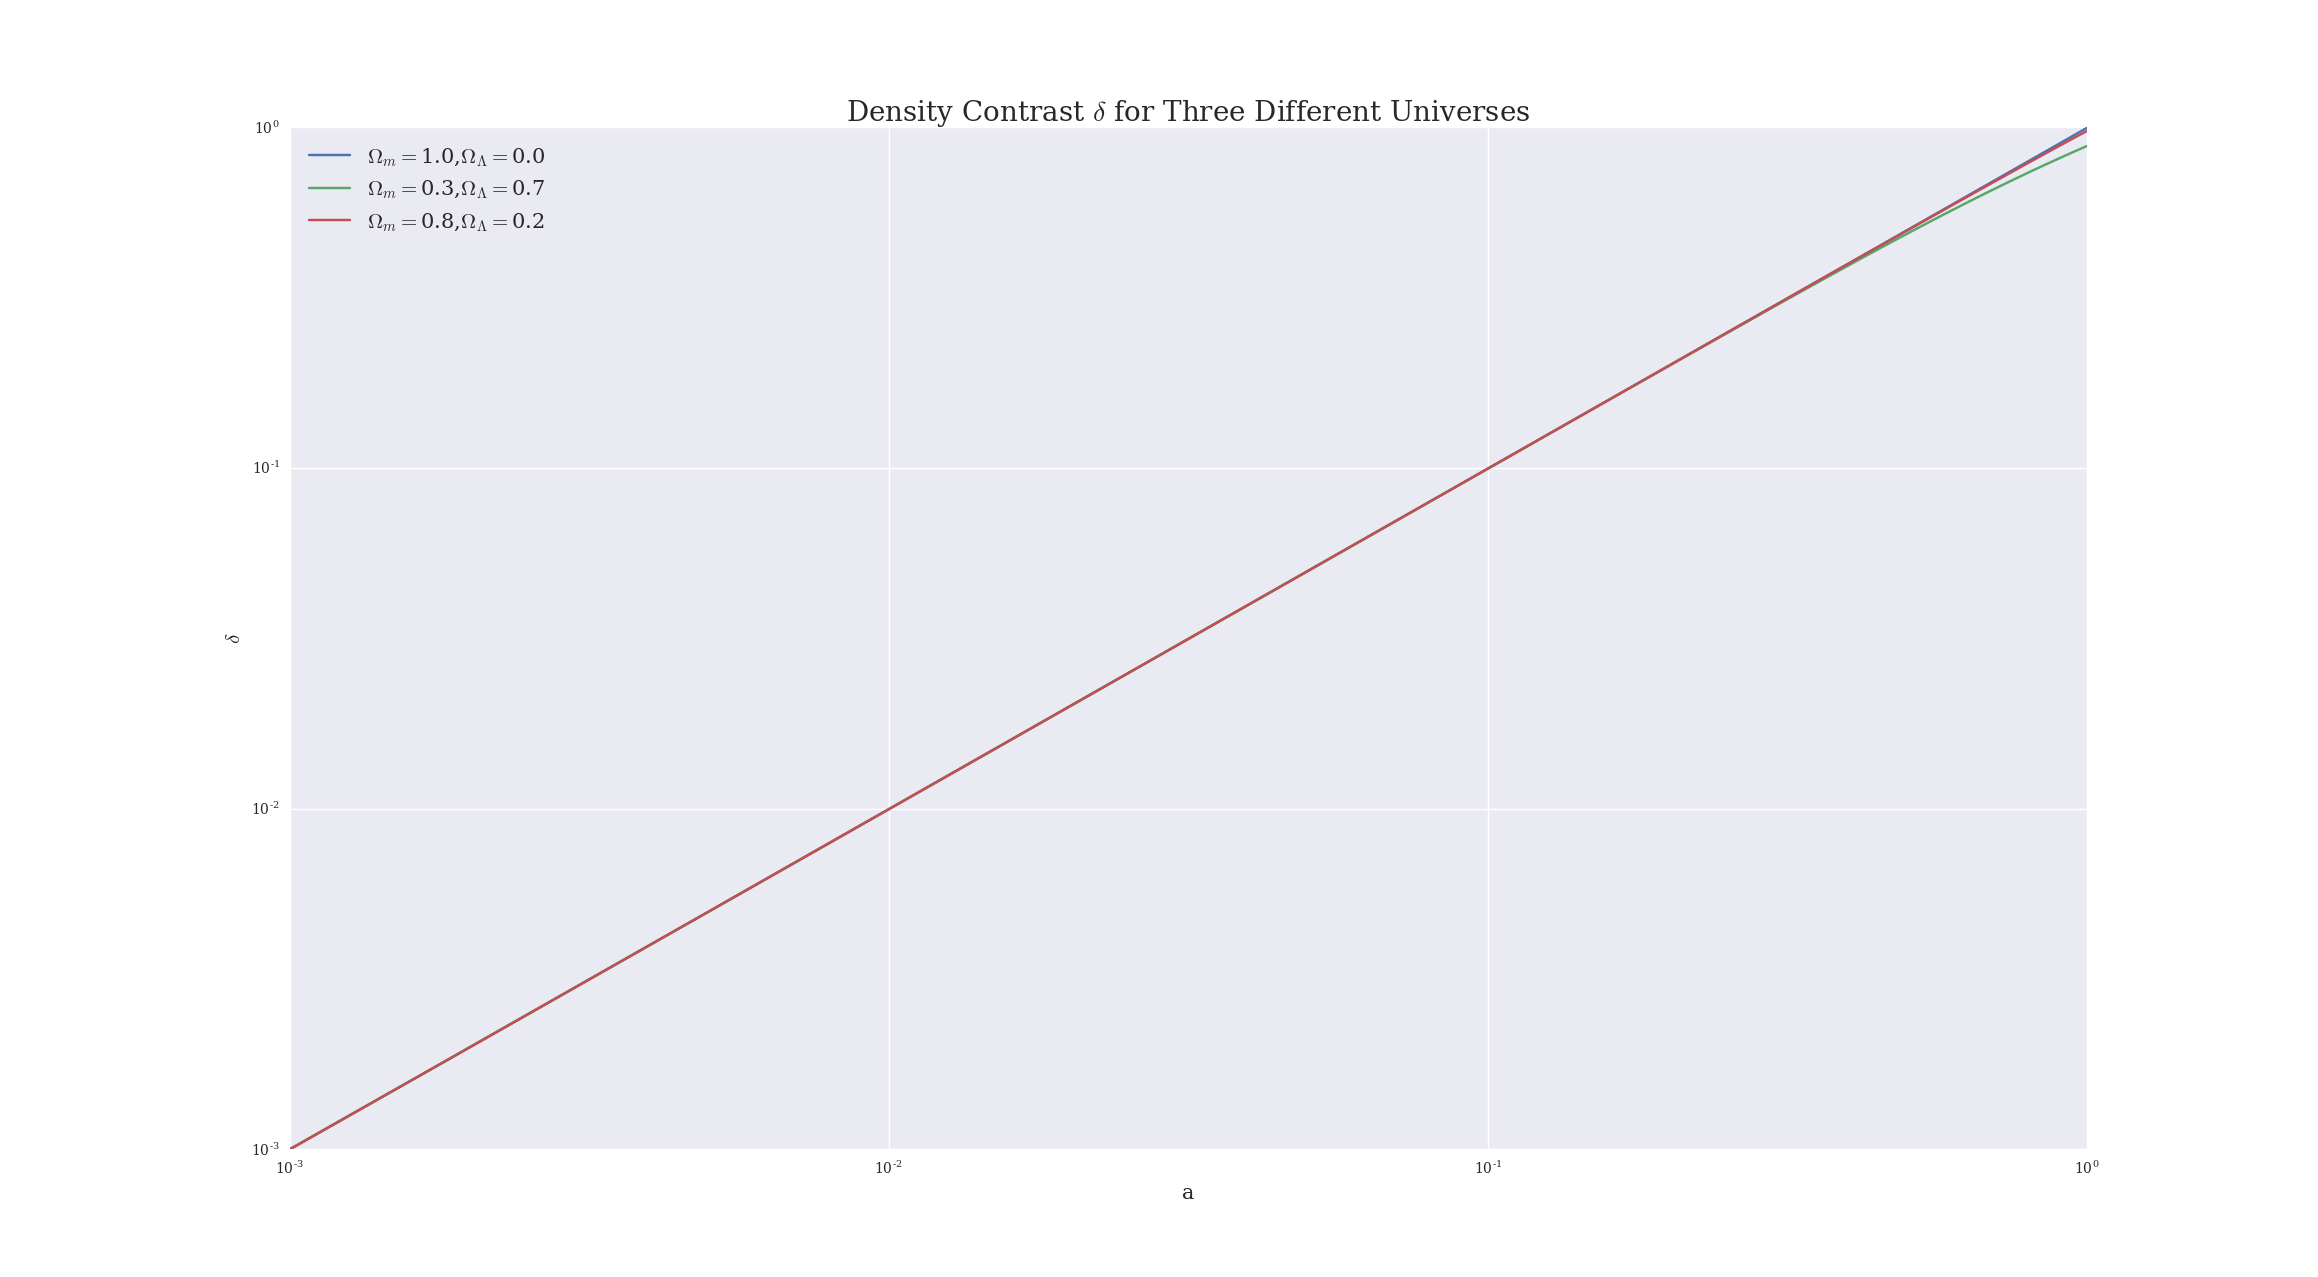
\includegraphics[scale=0.25]{a_v_delta}
\caption{The evolution of the density contrast for three different universe models with only matter and a cosmological constant.}\label{fig:a_v_delta}
\end{figure}


We see from \ref{fig:a_v_delta} that for $(1,0)$ we have a linear function, which makes sense since we know that in this universe $\delta \propto a$. For the other two universes we see that $\delta \propto a$ for most of the time. This is due to matter being dominant in the early universe. But later the the cosmological constant takes over, and we get a more rapid expansion. Due to the rapid expansion of $\Lambda$ structures will have a more difficult time forming, and will more likely be torn apart. We therefore see that $\delta$ decreases. The larger $\Omega_{\Lambda}$ is the more expansion there will be, and $\delta$ will decrease faster.

\subsection{c)}
We now want to find the grown factor 
\begin{equation}\label{eq:f}
f = \frac{\ln \delta}{\ln a}.
\end{equation}
Since we have $\delta$ and $a$, we can approximate this numerically as
\begin{equation}
f_{i+1} \approx \frac{\Delta \ln \delta}{\Delta \ln a} = \frac{\ln \delta_{i+1} - \ln \delta_{i}}{\ln a_{i+1} - \ln a_{i}} = \frac{\ln \frac{\delta_{i+1}}{\delta_{i}}}{\ln \frac{a_{i+1}}{a_{i}}}.
\end{equation}
This is straight forward to calculate. We can then plot it against the redshift
\begin{equation}
z = \frac{1}{a} - 1.
\end{equation}

\begin{figure}[!h]
\centering
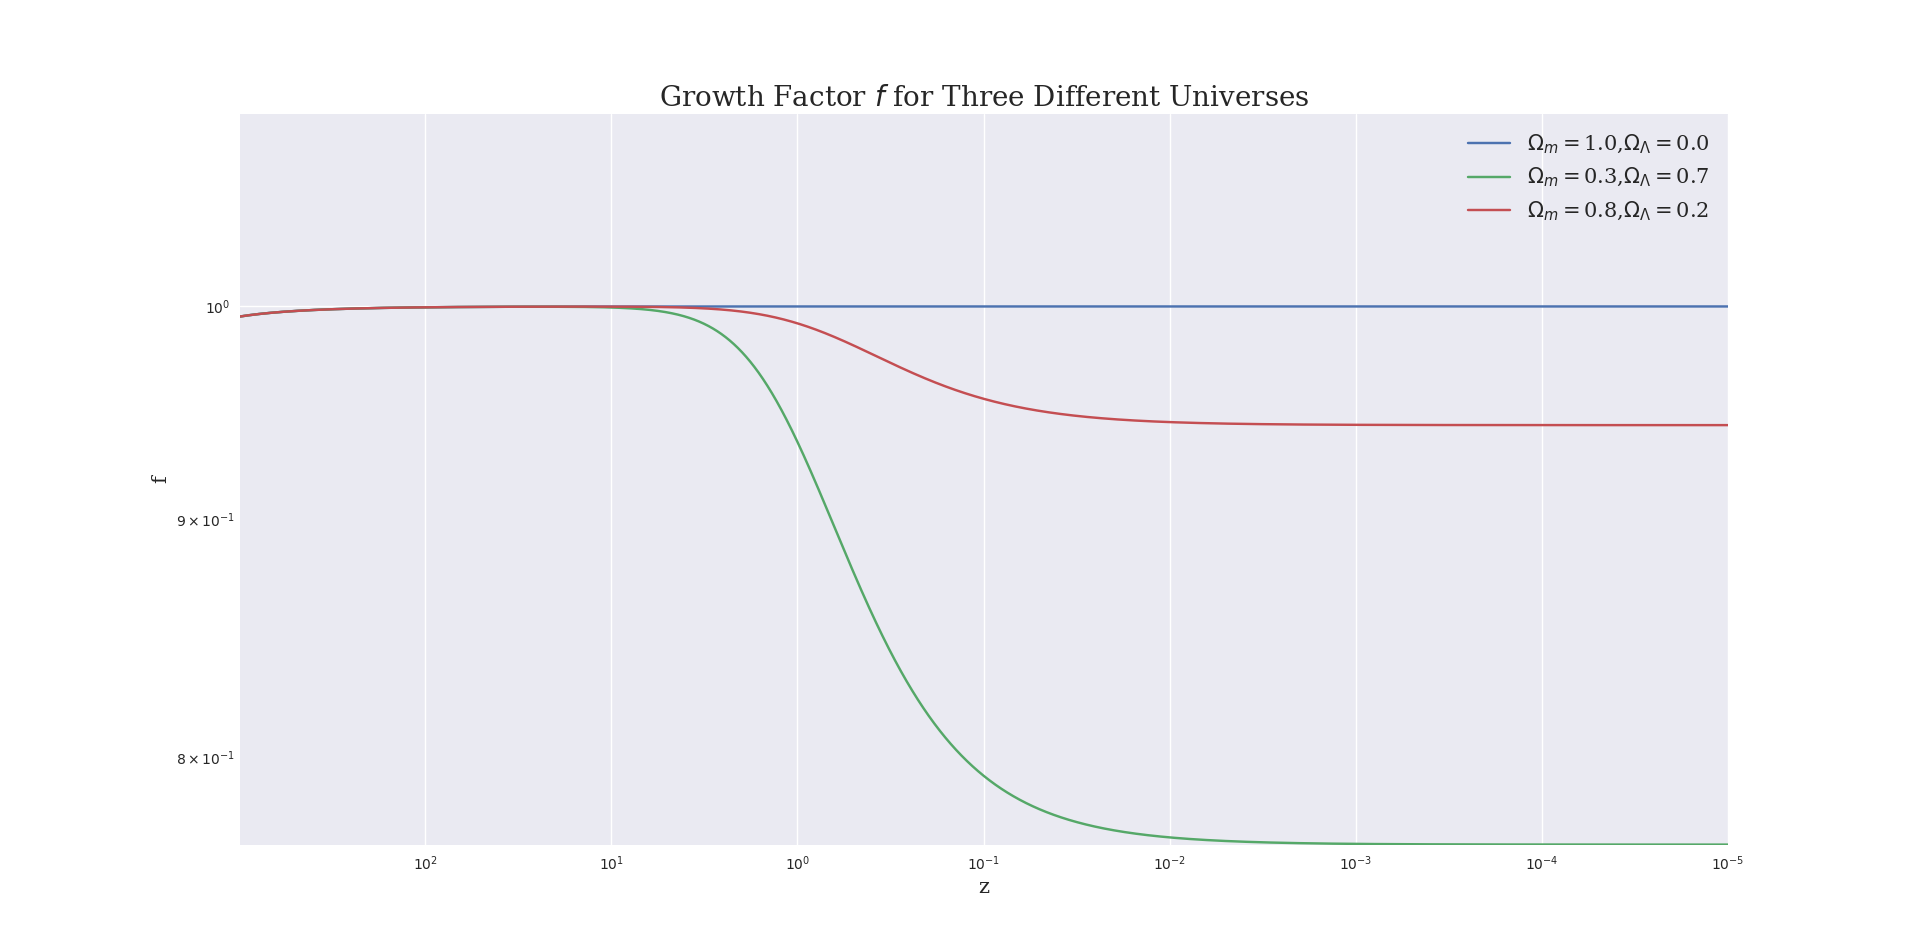
\includegraphics[scale=0.25]{z_v_f}
\caption{The evolution of the growth factor for three different universe models with only matter and a cosmological constant.}\label{fig:z_v_f}
\end{figure}

As we see from \ref{fig:z_v_f} the growth factor for the $\Omega_{m} = 1$ universe is more or less flat at $f = 0$. The two other models again follows this at the early stages, but decreases for lower $z$, with the model with highest $\Omega_{\Lambda}$ decreasing most.

\section{Exercise 3}
\subsection{a)}
We start with the temperature for the gas. Since we have a adiabatic expansion, we start with an adiabatic expression for the temperature and volume of a gas
\begin{equation}
TV^{\gamma - 1} = C,
\end{equation}
where $T$ is the temperature, $V$ the volume, $C$ a constant and $\gamma$ is the degrees of freedom, given for a monoatomic gas as $\gamma = 5/3$. We also know that the volume has to be $V \propto a^{3}$, so
\begin{equation}
T_{gas} = \frac{C'}{(a^3)^{5/3 - 1}} = C'a^{-2}.
\end{equation}
($C'$ is some constant). 

For the gas we start with Wien's displacement law for a black body
\begin{equation}
T = \frac{b}{\lambda},
\end{equation}
where $\lambda$ is the wavelength and $b$ a constant (it's value is known, but uninteresting here). We know that $\lambda \propto a$ so
\begin{equation}
T_{\gamma} = Ba^{-1}.
\end{equation}

We know that at the point of decoupling, the temperature must have been the same. This happen at $z = 1100 \Rightarrow a \approx 10^{-3}$ with the temperature $T = 4000K$. Using this we find the constants for the temperatures, and find the temperatures evolves like
\begin{equation}
T_{gas} = 4\cdot 10^{-3}a^{-2}, \quad T_{\gamma} = 4a^{-1}.
\end{equation}

\begin{figure}[!h]
\centering
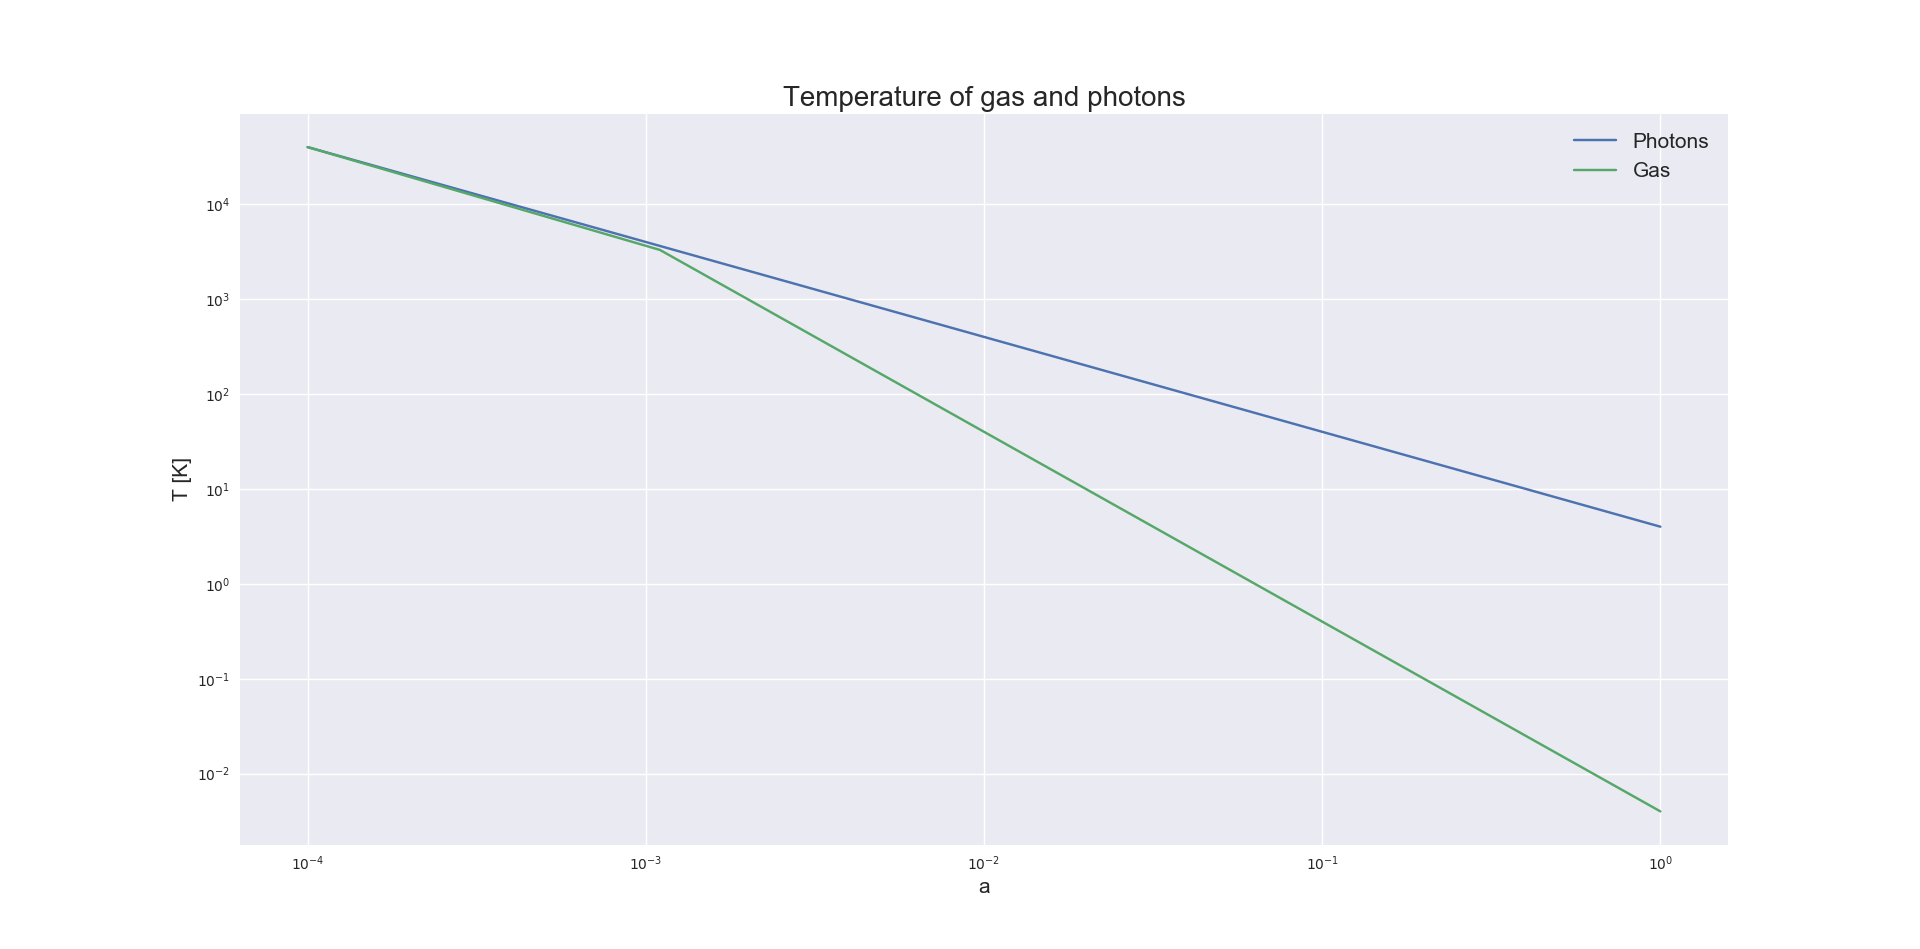
\includegraphics[scale=0.25]{temp}
\caption{The evolution of the temperature of the gas and photons found in the universe.}\label{fig:temp}
\end{figure}

We see from \ref{fig:temp} that the temperature were the same before decoupling\footnote{Hard coded to be that way...}. After decoupling the temperature of the gas decrease much faster due to its dependence on $a^{-2}$, with the photons decreasing less to their dependence on $a^{-1}$. 

\subsection{b)}
We now want to look at the Jeans length and mass. They are generally given as
\begin{equation}
\lambda_{J} = c_{s}\sqrt{\frac{\pi}{G \rho}}, \quad M_{J} = \frac{\pi^{5/2}}{6G^{3/2}\rho^{1/2}}\cdot c_s^{3}.
\end{equation}
The difference in these quantities before and after decoupling comes from the sound speed $c_s$. Before decoupling the gas is coupled with the photons, thus the sound speed is just $c/\sqrt{3}$, which is constant. For a gas we can find the sound speed as a function of redshift
\begin{equation}
c_s = \sqrt{\frac{k_b T}{\mu m_p}} = \sqrt{\frac{k_b}{\mu m_p}}T^{1/2} = \sqrt{\frac{k_b}{\mu m_p}}\left(4\cdot 10^{-3}a^{-2}\right)^{1/2} = 4\cdot 10^{-3/2}(1+z)\sqrt{\frac{k_b}{\mu m_p}},
\end{equation}
where $k_b$ is Boltzmann's constant, $m_p$ is the proton mass and $a = 1/(1+z)$. We are going to use that $\rho = \rho_0 a^{-3}$, we thus get that 
\begin{equation}
\rho = \rho_0 (1+z)^3.
\end{equation}
We can then write the Jeans mass and length as functions of redshift
\begin{equation}
\lambda_{J,after} = 4\cdot 10^{-3/2}(1+z)(1+z)^{-3/2}\sqrt{\frac{k_b}{\mu m_p}}\sqrt{\frac{\pi}{G \rho_0^{1/2}}} =4\cdot 10^{-3/2}(1+z)^{-1/2} \sqrt{\frac{k_b}{\mu m_p}}\sqrt{\frac{\pi}{G \rho_0^{1/2}}}
\end{equation}
\begin{equation}
M_{J,after} = \frac{\pi^{5/2}}{6G^{3/2}\rho_0^{1/2}}\cdot \left(4\cdot 10^{-3/2}(1+z)\right)^{3}\cdot (1+z)^{-3/2} = 12\cdot 10^{-1/2}\frac{\pi^{5/2}}{6G^{3/2}\rho_0^{1/2}}(1+z)^{3/2}.
\end{equation}
This is after the decoupling. Before decoupling the only dependence on redshift comes from the density, so we get
\begin{equation}
\lambda_{J,before} = \frac{c}{\sqrt{3}}\sqrt{\frac{\pi}{G \rho_0}}(1+z)^{-3/2}
\end{equation}
\begin{equation}
M_{J,before} = \frac{\pi^{5/2}}{6G^{3/2}\rho_0^{1/2}}\cdot \left(\frac{c}{\sqrt{3}}\right)^3\cdot(1+z)^{-3/2}.
\end{equation}


\begin{figure}
     \centering
     \subfloat[][a]{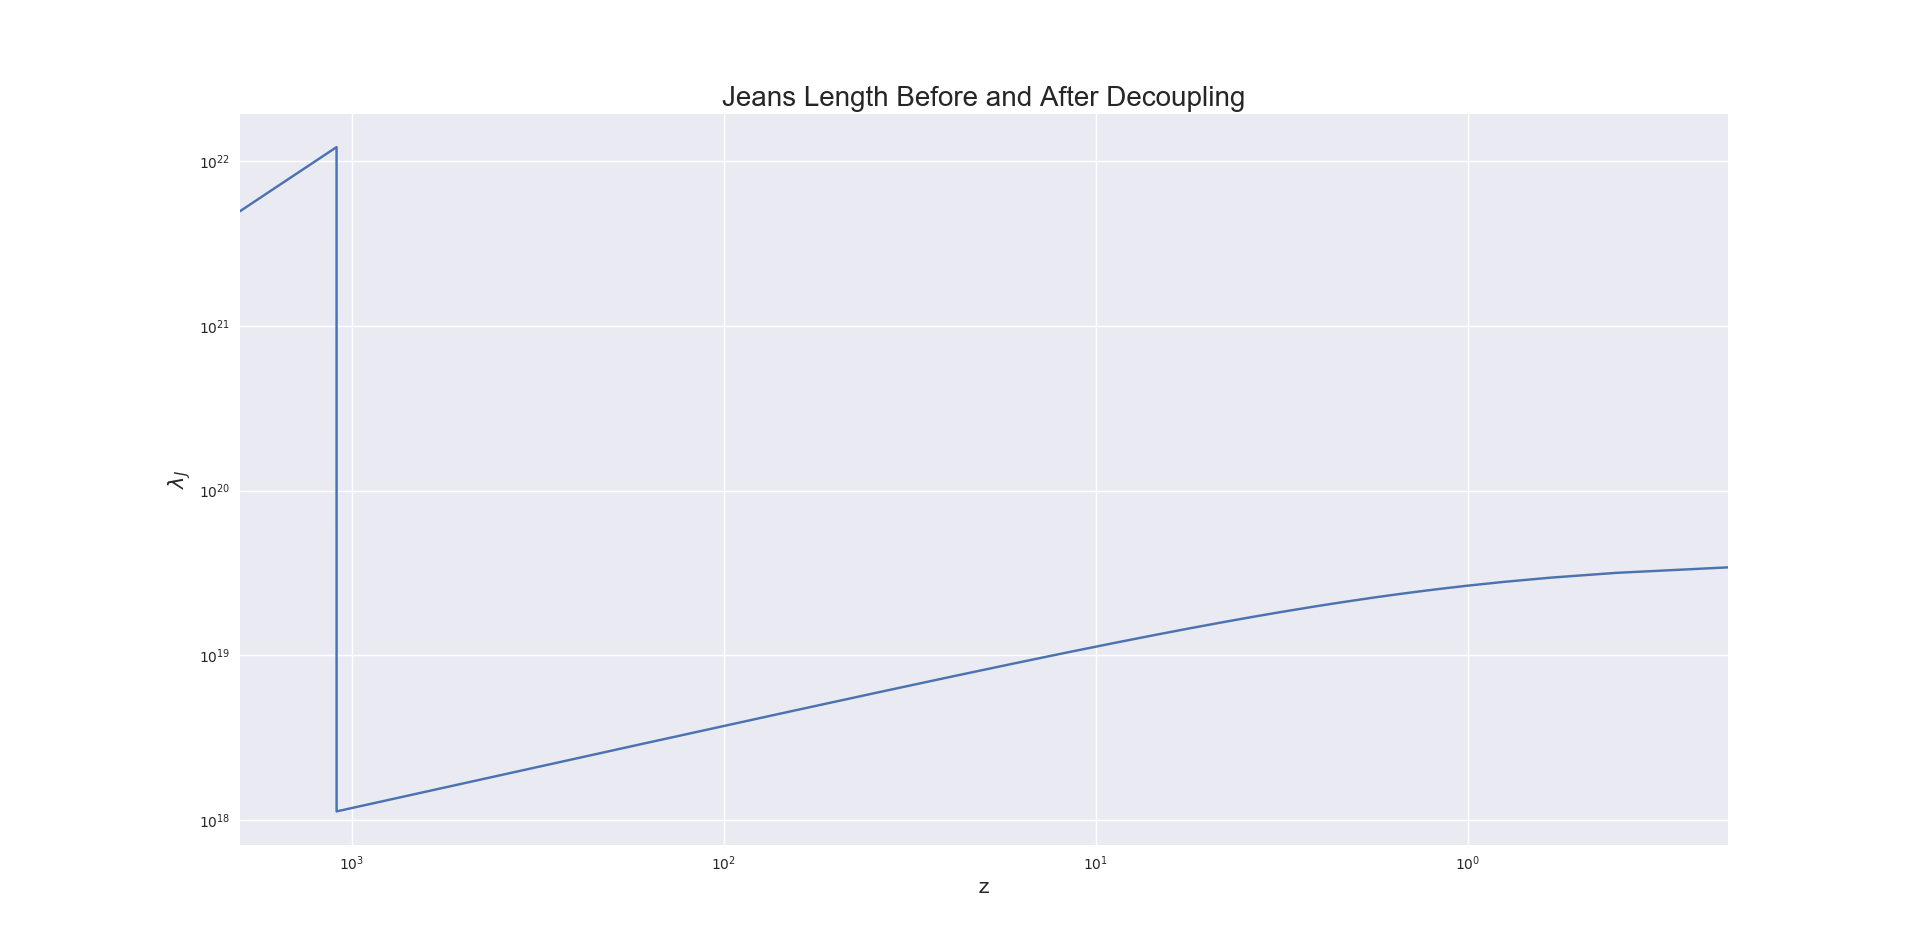
\includegraphics[scale=0.12]{length}\label{fig:length}}
     \subfloat[][b]{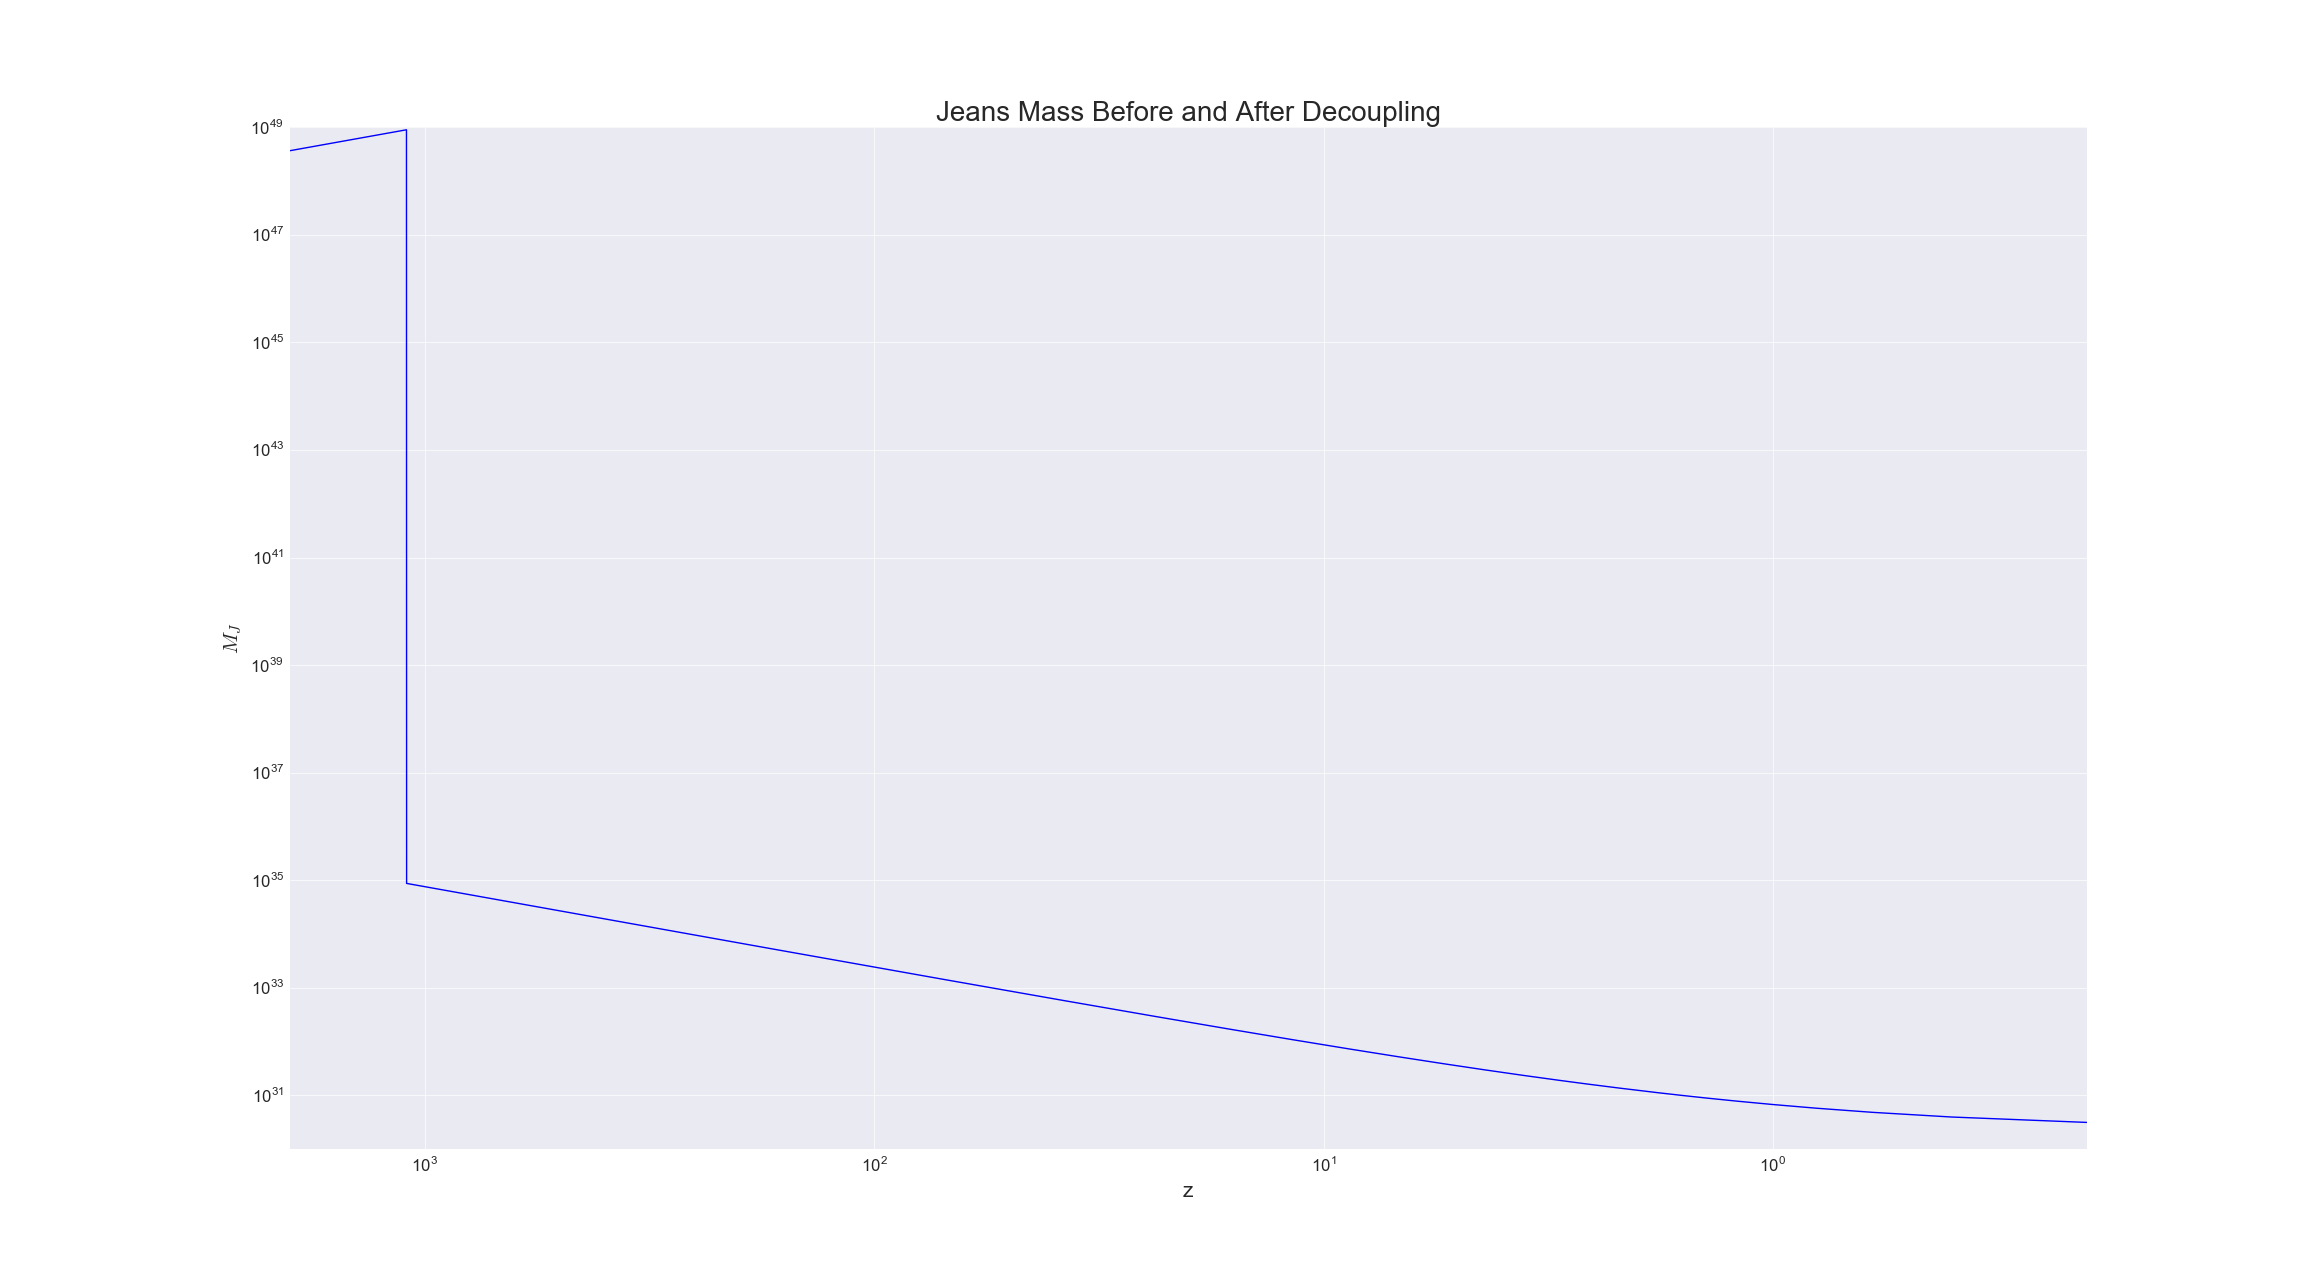
\includegraphics[scale=0.12]{mass}\label{fig:mass}}
     \caption{Comparison of steady state results (a) x method (b) y method}
     \label{steady_state}
\end{figure}


\section{Exercise 4}



We have the differential equation 
\begin{equation}\label{eq:Rdotdot}
\ddot{R} = -\frac{GM}{R^2},
\end{equation}
and the parametric solutions 
\begin{equation}\label{eq:param}
R = A(1-\cos \theta), \quad t = B(\theta - \sin \theta), \quad A^3 = GMB^2.
\end{equation}
We start with eq. \eqref{eq:Rdotdot}, and multiply both sides with $dR/dt$
\begin{equation}
\frac{dR}{dt}\cdot \frac{d^2R}{dt^2} = - \frac{dR}{dt}\frac{GM}{R^2} \Leftrightarrow \frac{1}{2}\frac{d}{dt}\left(\frac{dR}{dt}\right) = \frac{d}{dt}\left(\frac{GM}{R}\right).
\end{equation}
Integrating on both sides gives us
\begin{equation}\label{eq:E}
\frac{1}{2}\left(\frac{dR}{dt}\right)^2 - \frac{GM}{R} = E,
\end{equation}
where $E$ is a constant (total energy). We are going to assume that $R$ and $t$ from \eqref{eq:param} are partially solutions to this differential equation. If this is correct, we should retrieve the relation between $A$ and $B$. Let us start be noting that
\begin{equation}\label{eq:dRdt}
\frac{dR}{dt} = \frac{dR}{d\theta}\frac{d\theta}{dt} = \frac{dR}{d\theta}\left(\frac{dt}{d\theta}\right)^{-1} = \frac{A\sin \theta}{B(1-\cos \theta)}.
\end{equation}
We then see that \eqref{eq:E} becomes
\begin{equation}\label{eq:E_param}
\frac{1}{2}\frac{A^2}{B^2}\frac{\sin^2 \theta}{(1-\cos \theta)^2} - \frac{GM}{A(1-\cos \theta)} = E.
\end{equation}
$E$ is constant, so it has the same value for all values of $\theta$. So to find its value, we choose to check it at $\theta = \pi$, with gives $\sin \theta = 0$ and $\cos \theta = -1$
\begin{equation}
E = 0 - \frac{GM}{A(1+1)} = -\frac{GM}{2A}.
\end{equation}
We can now input this into eq. \eqref{eq:E} to get
\begin{equation}
\frac{1}{2}\frac{A^2}{B^2}\frac{\sin^2 \theta}{(1-\cos \theta)^2} - \frac{GM}{A(1-\cos \theta)} = -\frac{GM}{2A}
\end{equation}
\begin{equation}
\Rightarrow \frac{1}{2}\frac{A^2}{B^2}\frac{\sin^2 \theta}{(1-\cos \theta)^2} = -\frac{GM}{2A}\left(1 - \frac{2}{1-\cos \theta)}\right).
\end{equation}
Then note that
\begin{equation}
\frac{\sin^2 \theta}{(1-\cos \theta)^2} = - \left(1 - \frac{2}{1-\cos \theta)}\right) = \cot^2\left(\frac{\theta}{2}\right),
\end{equation}
which gives us
\begin{equation}
\frac{A^2}{B^2} = \frac{GM}{A} \Leftrightarrow A^3 = GMB^2.
\end{equation}
This retrieves the relation from eq. \eqref{eq:param}. This means that the parameterized equations are solutions to \eqref{eq:E} which again means they are solutions to \eqref{eq:Rdotdot}.

\section{Exercise 5}
From the definition of $v$ and what we calculated in \eqref{eq:dRdt}, we see that
\begin{equation}
v = \frac{dR}{dt} = \frac{A\sin\theta}{B(1-\cos \theta)} \Rightarrow v^2 = \frac{A^2}{B^2}\frac{\sin^2 \theta}{(1-\cos \theta)^2}.
\end{equation}
The last step is just to make it easier later. We want to find to find the velocity at the virial radius, which we know is $R_{vir} = 0.5R_{max}$. For the parameterized solution, we know that $R_{max} = 2A$, which gives $R_{vir} = A$. From the definition of $R$ we get that
\begin{equation}
R = A(1-\cos \theta) = A \Rightarrow \theta = \pi \text{ or } \frac{3\pi}{2}. 
\end{equation}
Since the virialization don't happen before $R_{max}$ we must have that
\begin{equation}
\pi_{vir} = \frac{3\pi}{2}.
\end{equation}
This gives us $\sin \theta = 1$, so we get
\begin{equation}
v^2 = \frac{A^2}{B^2} = \frac{A^2}{\frac{A^3}{GM}} = \frac{GM}{A}.
\end{equation}
We know that $R_{vir} = A$, so we get out answer
\begin{equation}
v_{infall} = \sqrt{\frac{GM}{R_{vir}}}
\end{equation}

\section{Exercise 6}
The gravitational binding energy is found in the following way\footnote{To not be called out on plagiarism, this derivation is heavily inspired by/stolen from \url{https://en.wikipedia.org/wiki/Gravitational_binding_energy} and \url{http://scienceworld.wolfram.com/physics/SphereGravitationalPotentialEnergy.html}}:

The energy needed to escape from a system is the same as peeling away all the mass of the system, layer by layer and letting them go to infinity. The energy required to do this is the binding energy. So the energy of peeling one layer is thus given as
\begin{equation}
dU = - G\frac{m_{shell}m_{interior}}{r}.
\end{equation}
The mass that resides in the interior under the shell, is simply that of a sphere
\begin{equation}
m_{interior} = \frac{4}{3}\pi r^3 \rho.
\end{equation}
The shell has a volume equal to that of the area of a sphere times the infinitesimal thickness of said shell. This gives us the mass
\begin{equation}
m_{mass} = 4\pi r^2\rho dr.
\end{equation}
These give us
\begin{equation}
dU = - G\frac{\frac{4}{3}\pi r^3 \rho\cdot 4\pi r^2\rho dr}{r} = -G\frac{16}{3}\pi^2\rho^2 r^4 dr.
\end{equation}
To get the total energy, we simply integrate from $r=0$ to the edge of the mass $r=R$
\begin{equation}
U = -\frac{16}{3}G\pi^2\rho^2 \int_0^R r^4 dr = -\frac{16}{15}G\pi^2\rho^2 R^5.
\end{equation}
For a uniform sphere with radius $R$, the density $\rho$ is simply given as
\begin{equation}
\rho = \frac{M}{4/3 \pi R^3}.
\end{equation}
This gives us the binding energy
\begin{equation}
U = -\frac{3GM^2}{5R}.
\end{equation}




\end{document}


